\documentclass[%
 reprint,
 amsmath,amssymb,
 aps,
 pra,
]{revtex4-1}

\usepackage{graphicx}% Include figure files
\usepackage{dcolumn}% Align table columns on decimal point
%\usepackage{bm}% bold math
\usepackage{fullpage}
\usepackage{epsfig}
\usepackage{amsmath}
\usepackage{amsthm}
\usepackage{amsfonts}
\usepackage{amssymb}
\usepackage{float}
\usepackage{pstricks}
\usepackage{cancel}
\usepackage{lipsum}
%\usepackage[nottoc,numbib]{tocbibind} %Uncomment for bibliography to be its own numbered section
\usepackage{units}
\usepackage{listings}
\usepackage{xfrac}
\usepackage{subcaption}

\graphicspath{{./plots/}}

\begin{document}

\preprint{APS/123-QED}

\title{\textbf{Lab Report: Phase Transitions} \\ \small{An Investigation of The VO$_2$ Metal-Insulator and BaTiO$_3$ Ferroelectric Transitions}}
\author{Joshua LaBounty}
\author{Thomas Krahulik}
\affiliation{Stony Brook University --- PHY 445}

\date{\today}

\begin{abstract}
	In this experiment, we explore the properties of the first order metal-insulator transition of VO$_2$ and the second order ferroelectric transition of BaTiO$_3$. We do this by measuring the voltage across these samples as they are heated above and beyond the critical temperatures ($T_C$). We use these experiments to explore and verify important foundations of phase transition theory, such as the Curie-Weiss law, and to compare our data to known values.
\end{abstract}
\maketitle

\section{Introduction}

Like gravity, phase transition are phenomena which have long been observed, but only recently have they been understood scientifically. The freezing, melting, and evaporation of water has long been central to human life, controlling the availability of food and the need for shelter, but only in the past two centuries has any real effort been put into a scientific understanding of how matter transitions between these phases. The first serious attempt to understand this type of phenomenon was undertaken by Charles Caignard de la Tour in 1822. In his study, he classified the 'solid $\leftrightarrow$ liquid $\leftrightarrow$ gas' phase transitions of alcohol according to the Temperature, Pressure, and Volume at which they occurred \cite{phase_history}. Later, in 1873, Josiah Willard Gibbs built on this work to introduce the concept of the phase diagram\cite{phase_history, gibbs}. With this diagram came the notion that phase transitions could be understood from a purely thermodynamic perspective. And, with the discovery of the ferromagnetic phase transition by Peter Curie in 1895 (along with its formal description by Peter Weiss in 1907), the race was on to find and classify phase transitions in a wide variety of systems. However, it wasn't until the discovery of the phase transition of liquid helium to a superfluid state that a solid classification system was able to take hold. It was observed experimentally that, during this transition, there was no latent heat and no visible boundary between the two phases \cite{phase_history}. Instead, it was found that there was a discontinuity in the second derivative of the free energy of the system, which showed itself in the famous lambda plot of heat capacity vs. temperature (Figure \ref{fig:lambda_point_helium}). This observation spurred Ehrenfest to introduce the first comprehensive classification system for phase transitions. The system was constructed around the 'order' of the discontinuity of the free energy of the system. Classically known phase transitions (water $\leftrightarrow$ ice, etc.) as well as others like the ferromagnetic transition of iron he classified classified as first order phase transitions, while the newly discovered HeI $\leftrightarrow$ HeII transition was a second order transition \cite{physics_of_phase, manual}. This classification scheme was soon validated, as superconductivity was proven to accompany the helium superfluid transition in the second order category. Landau built on this classification system to create much of the theory of phase transitions we still use today \cite{manual}.

\begin{figure}[H]
	\centering
	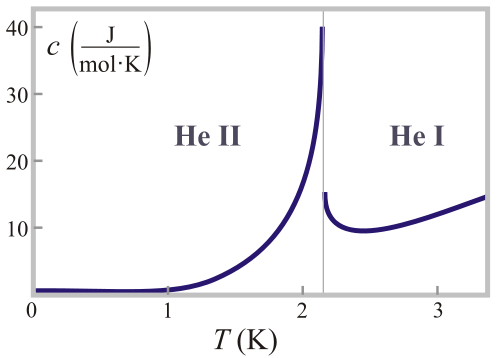
\includegraphics[width=0.3\textwidth]{lambda.png}
	\caption{Diagram showing the discontinuity in the heat capacity of liquid helium. Image courtesy of Wikimedia Commons.}
	\label{fig:lambda_point_helium}
\end{figure}

The two main types of phase transitions, and the only two we concern ourselves with here, are phase transitions of the first and second order. Third and higher order transitions exist, but are much less common than either of the lower orders \cite{thirdorder}. First order transitions, as stated above, are characterized by a discontinuity in the derivative of the free energy. This gives rise to two different functions for the free energy, $F_1$ and $F_2$, above and below the critical temperature $T_C$ \cite{manual, physics_of_phase}. If there were no energy cost to the material switching between the two phases, we would expect to see the phase transition of the entire material occur at exactly $T_C$. However, because the transition between phases often involves a physical rearrangement of the system, there must be some energy cost. Because of this, local energy minima can form (and remain stable for a good deal of time) where the original phase exists even above $T_C$. Extra heat is required to overcome the energy of the kinetic barrier between the regions of differing phases, and so the transition will happen at $T_C + T^*$ \cite{manual}. The same phenomenon occurs when cooling, and the transition will take place at $T_C - T^*$. This will result in a hysteresis curve. We study this first order hysteretic phenomenon in Vanadium Dioxide (VO$_2$), which undergoes a first order Metal-Insulator transition.

Second order transitions, by contrast, have a continuous function of $F$ across all temperature ranges (barring the material being subject to an unrelated first order transition). Thus, from the transition, there is no change in latent heat ($Q = 0$) and $\Delta U = 0$ \cite{manual}. Thus, we have an order parameter which is $0$ at $T_C$ and increases as $T$ moves away from $T_C$. This fact allowed Landau to construct his theory of second order phase transitions by expanding $F(T)$ as a function of the order parameter $m$ in the vicinity of $T_C$ \cite{manual, phase_1}. Omitting odd powers in the expansion due to symmetry considerations \cite{manual}, the expression reads:
\begin{gather}
	\begin{align}
	F\left(T\right) 	& = F_0\left(T\right)+\alpha(T) m^2+\frac{1}{2}\beta(T) m^4 \nonumber \\
	\downarrow 		& ~~~~~~~~~~~~~~~ \frac{d^2F}{dm^2} > 0 \nonumber \\
					& =F_0\left(T\right)+\alpha_0(T - T_C) m^2+\frac{1}{2}\beta_0 m^4 \nonumber
	\end{align}
\end{gather}
In order to find the value of the order parameter corresponding to the phase transition, we wish to minimize this function with respect to $m$. Doing this, we find that:
\begin{gather}
	m = 	\begin{cases}
			0 & T > T_C \\
			\pm \sqrt{\frac{\alpha_0 (T_C - T)}{\beta_0}} & T \le T_C
		\end{cases} \nonumber
\end{gather}
Physically, this means that above the critical temperature, there is only one state for the system to be in, which corresponds to $m = 0$. Below the critical temperature, this symmetry is broken into two states, one with $+m$ and one with $-m$, each with its own stable minima of $F(T)$. We will measure this parameter, and relate it to important quantities like succeptability $\chi$ and the Curie-Weiss constant, later in the lab. The second order transition we will be studying is the ferroelectric transition of Barium Titanate (BaTiO$_3$) due to its perovskite crystal structure.

\section{Review of Previous Work}

Phase transitions have long been the subject of intense study, and their importance to solid-state physics and materials science cannot be overstated. Early studies of the phase transitions of alcohol paved the way for thermodynamics as we know it to take shape \cite{phase_history}. More recently, phase transitions have been used successfully in a wide variety of industrial applications.

The superconducting phase transition is the subject of much study, and with good reasons. Superconductors have applications ranging from the construction of magnets \cite{magnets} to the construction of magnetic cloaks \cite{rapheal}, from quantum computers \cite{quantum_super, quantum_super2} to trains \cite{trains} --- the list is endless. And understanding the phase transition of superconductors is the first step in being able to harness their unique abilities. The superconducting transition is of the second order, and much painstaking effort has been taken to understand the theory of the transition exactly (beyond the mean field approach allowed by the Ginzburg-Landau model) \cite{superconductor, supercond2, supercond3}.

The applications of the metal-insulator transition, studied here, is itself far reaching. It has been shown that an ultra-fast electronic switch can be constructed from vanadium dioxide (among other MIT materials) \cite{switching}. Its applications also extend beyond this into computer memory and optical shutters \cite{memory}, as the MIT also changes the transparency of VO$_2$ to infrared light.

Barium Titanate, too, has many applications in electronics. It has long been used in the constuction of capacitors, particularly those where a high dielectric constant is desired ($k \sim 7000$) \cite{capacitors}. Additionally, as we will show in the lab, the capacitance of a BaTiO$_3$ capacitor will drop as it is heated across its critical temperature. This can be useful for systems where a temperature dependent capacitance is desired. Because of its ferroelectric properties, Barium Titanate can also be used in a wide variety of thermal imaging systems, non-linear optics, and other advanced electronic devices \cite{thermals}.

The mathematical underpinnings of phase transitions have also been extended to describe a wide range of phenomena. In the earliest moments of the Universe, cosmologists believe that the cosmos underwent a period of superluminal inflation \cite{cosmo}. The cause of this inflationary period has been theorized to be a phase transition brought about by fluctuations in the Higgs field \cite{cosmo2, cosmo3, cosmo4, cosmo5}. Thus, the mathematical underpinnings we discuss here have wide ranging applications throughout the natural sciences.

\section{Experimental Setup}

Our experimental setup consists of three main components: a Princeton Applied Research Model 5209 lock-in amplifier, a sample chamber connected to a voltage controlled heating coil, and (during the resistance measurements) a limiting resistor. 

The lock-in, essentially, consists of a frequency generator and a measuring input which is tuned only to that specific frequency. It is capable of generating a signal at a very specific frequency and phase and holding it there with great precision. The readout is then tuned to that frequency alone, but it can also be set to measure this frequency at any phase with respect to the original. Phasor theory tells us that the voltages across resistors  will be in-phase with the driving frequency, while voltages across capacitors will be $90^\circ$ out of phase. Thus, by looking at the in-phase and out-of-phase components of the input signal with the lock-in, we can determine the voltage across the resistive and capacitive portions of the system respectively. We began each measurement by 'tuning' the lock-in. We did this by hooking the output directly up to the input with a BNC cable. We then activated the autotune function, which seeks to maximize the in-phase signal. After this cycle completed, we manually adjusted the phase settings until the out of phase signal was as close to zero as we could obtain. We then hooked up the resistive or capacitive sample as detailed below.

The samples are mounted in a sample chamber (shown in Figure \ref{fig:sample:inplace}) which consists of an insulated double-walled aluminum container with leads which run into it. Wires run through the insulated walls and terminated in double-prong connections to which the VO$_2$ and BaTiO$_3$ samples can be attached. These wires also run out of the sample chamber and have connections to which the lock-in can be attached to provide input. A heater is wrapped around the sample chamber which we directly control with a Staco Energy voltage source. A temperature sensor is also placed inside the sample chamber to monitor the internal temperature. Both the voltage from the lock-in and the temperature measurements are fed into a LabView program, which records the data in a format which can be read in by our analysis software ROOT.

In previous years, a temperature controller was used which could ramp the temperature of the system up and down automatically, and at a much slower rate, but this system was not used for our experiments. As such, our ramps may have occurred at a faster speed than was ideal, and an artificial hysteresis-like effect may be introduced in our measurements due to a lag between measured temperature and sample temperature. 

Depending on the quantity being measured, resistance or capacitance, the system is set up in one of two different ways.

\subsection{Resistance Measurements}

\begin{figure}[H]
	\centering
	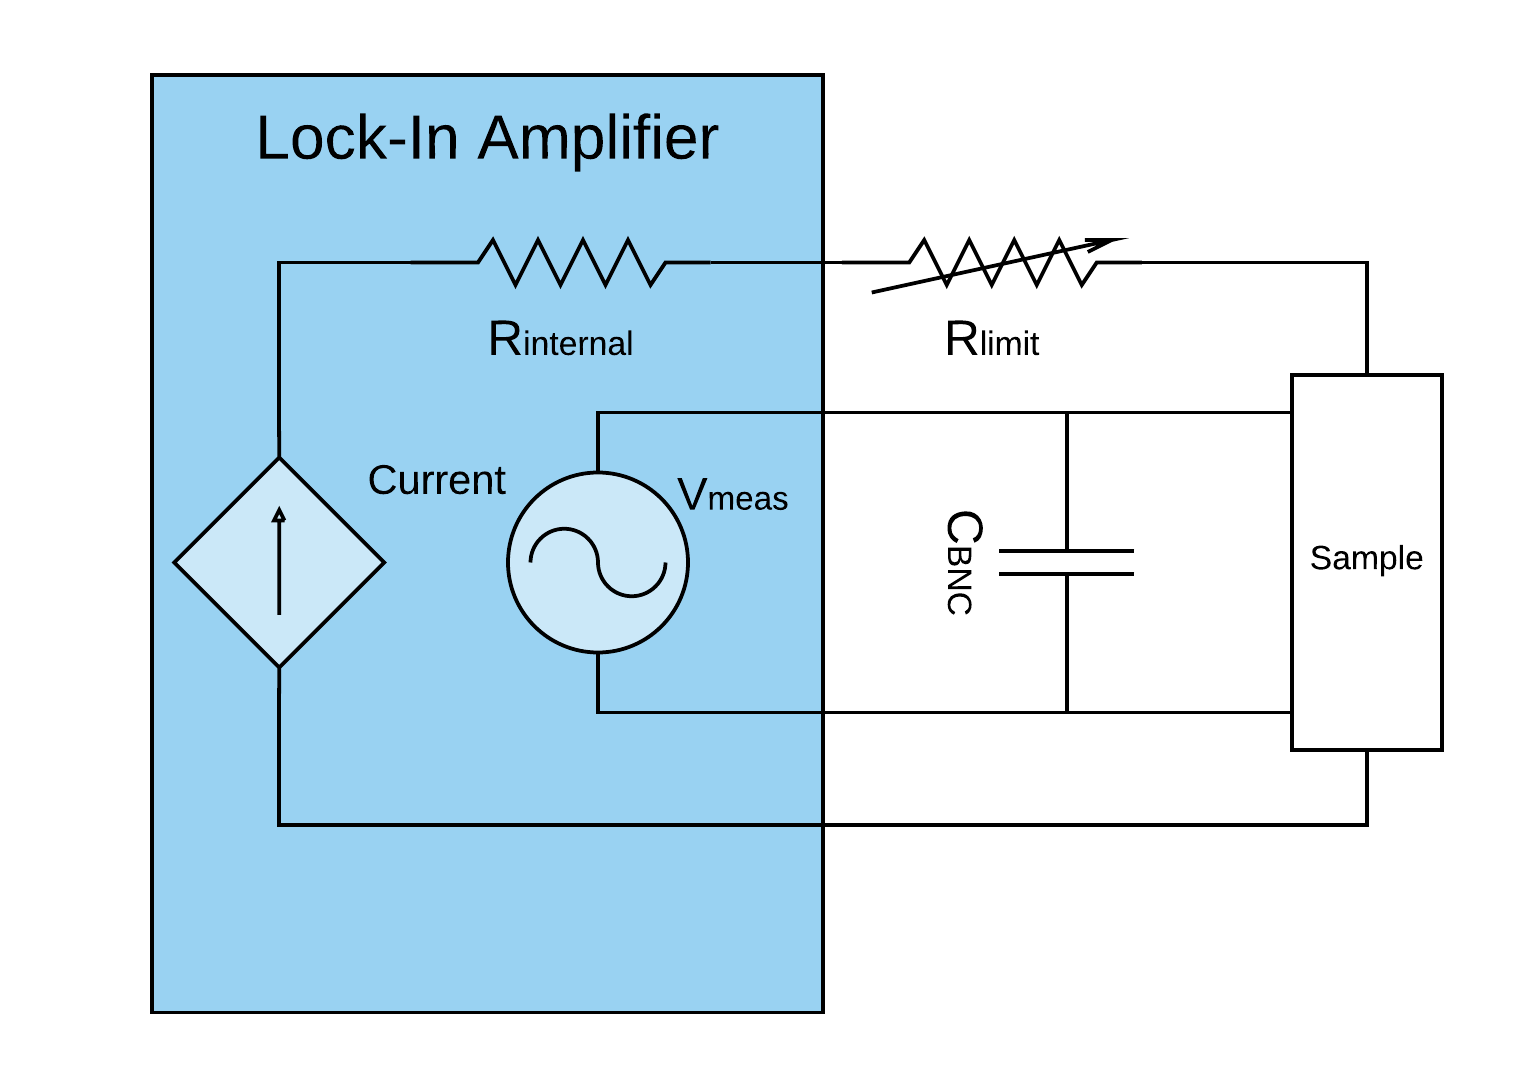
\includegraphics[height=5cm]{diagram_res.png}
	\caption{Circuit diagram showing the four-probe resistance measurement of a sample.}
	\label{fig:ResistanceMeasurements}
\end{figure}

For the resistance measurements, we set up the system as shown in Figure \ref{fig:ResistanceMeasurements}. We first connected the oscillator voltage out to a limiting resistor (a decade resistor set to $1~M\Omega$) in series with our sample, which was placed in the chamber. This was done to protect the delicate VO$_2$ sample from the potentially large currents which could otherwise pass through it. We then connected the sample to the input voltage leads In this configuration, known as the 'four-probe' resistance measurement method, the ammeter current does not pass through the contacts of the voltmeter. Thus the contact resistances do not effect out measurement to a large degree. A more in-depth explanation of this measurement method can be found in Appendix \ref{section:fourprobe}. We set the lock-in output to $V_{out} = 2.0~V$ and $\nu = 25~Hz$. The low frequency allows us to minimize the effect of the parasitic capacitance of the BNC cables (see Section \ref{section:factors}), as their reactance will be $X_C \sim 100~M\Omega$.

\subsection{Capacitance Measurements}

\begin{figure}[H]
	\centering
	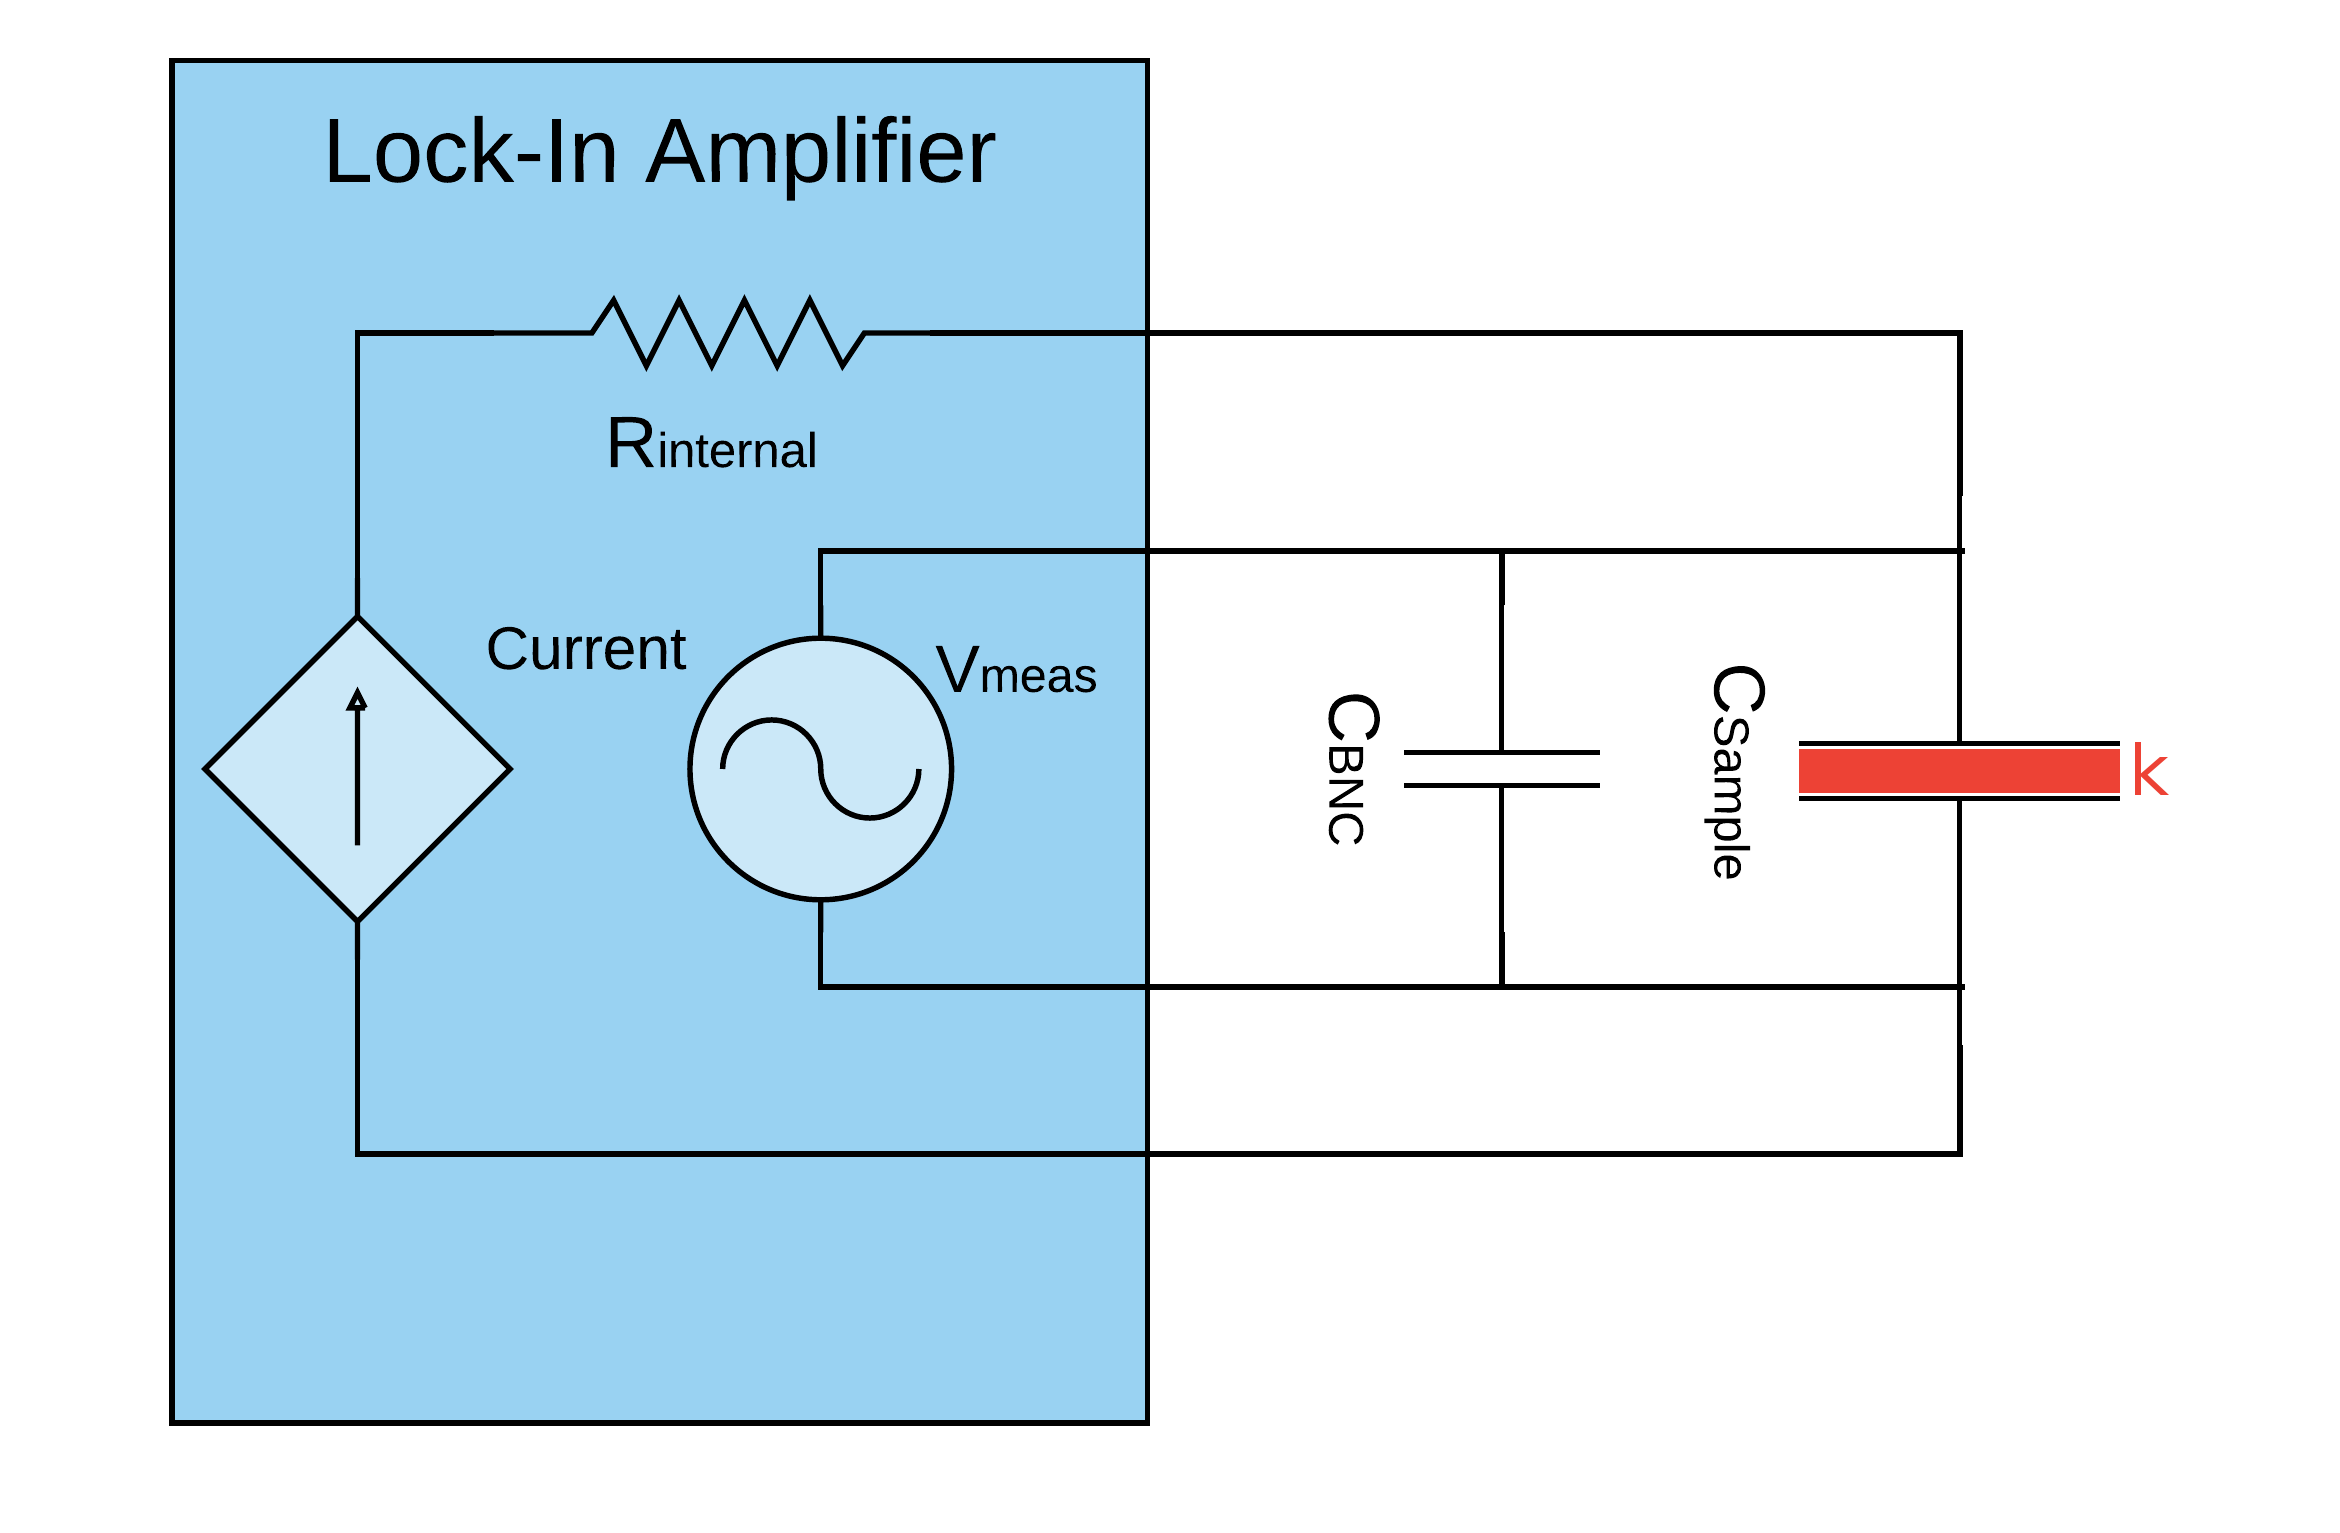
\includegraphics[height=5cm]{diagram_cap.png}
	\caption{Circuit diagram showing the measurement of the capacitance of a sample.}
	\label{fig:CapMeasurements}
\end{figure}

As opposed to the previous measurement, this setup does not make use of a limiting resistor, as the current through the sample will be nowhere near large enough to damage this capacitor. This also has the effect of making the (normally small) out-of-phase signal larger and thus easier to measure. The lock-in amplifier is also set to a much higher frequency for the capacitance measurements, $\nu = 25000~hZ$ rather than $25~Hz$. The rest of the setup remains unchanged, and a diagram of the lock-in portion can be seen in Figure \ref{fig:CapMeasurements}.

\subsection{Preparation of Samples}

Before we can take these measurements, however, we need to prepare the samples for measurement. In the course of this lab, we will make use of two different sample materials: Vanadium Dioxide (VO$_2$) and Barium Titanate (BaTiO$_3$). The Vanadium samples consist of a thin layer of VO$_2$ ($\sim 100~nm$) deposited on a silicon substrate. These Vanadium samples are pre-mounted on their electrical contacts, but we have prepared a Barium sample for our own use. Our goal with the Barium sample is to construct a parallel plate capacitor using silver paint on either side of a flat sample. In order to maximize the capacitance, in accordance with the known relation $C = \epsilon A/d$ where $\epsilon = k \epsilon_0$, we want to maximize the surface area of our sample and minimize its thickness. To that end, we chose the largest piece of Barium Titanate available and carved it down to a thin flat plate.

\begin{figure}[H]
	\centering
	\begin{subfigure}{0.22\textwidth}
		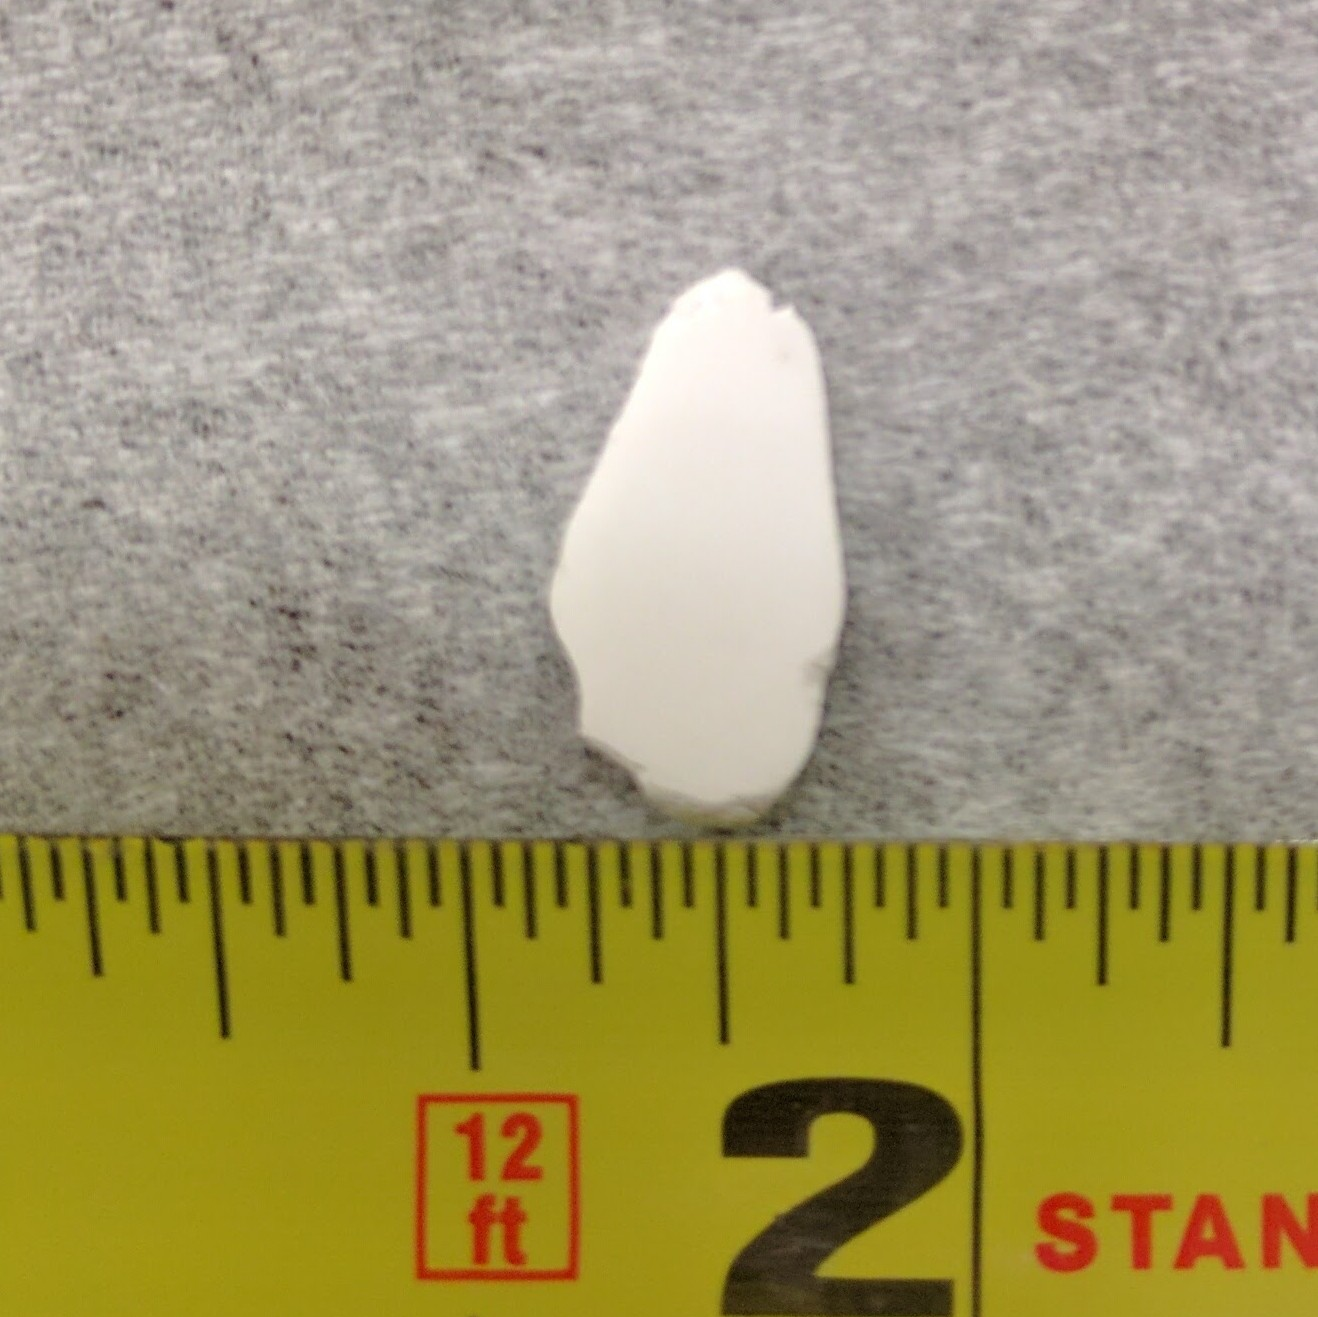
\includegraphics[width=1\textwidth]{sample_area.jpg}
		\caption{}
		\label{fig:sample:area}
	\end{subfigure}
	\begin{subfigure}{0.22\textwidth}
		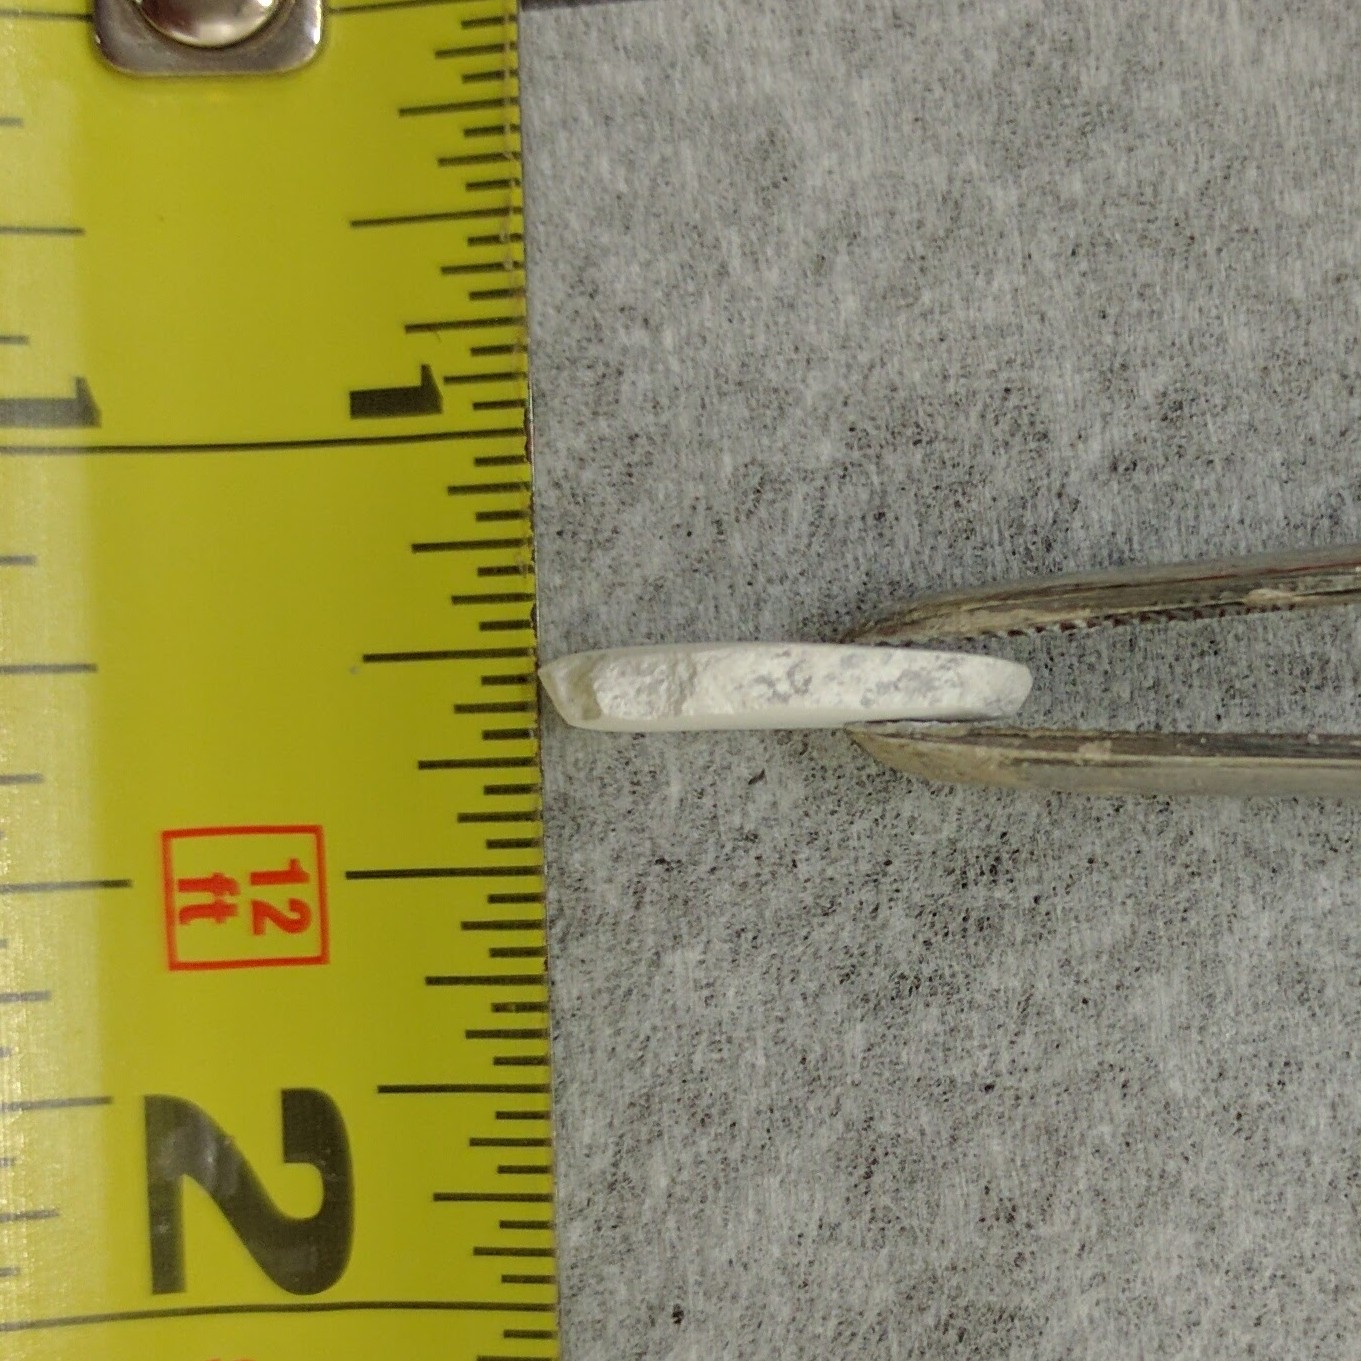
\includegraphics[width=\textwidth,angle=90]{sample_thickness.jpg} 
		\caption{}
		\label{fig:sample:thickness}
	\end{subfigure}
	\begin{subfigure}{0.22\textwidth}
		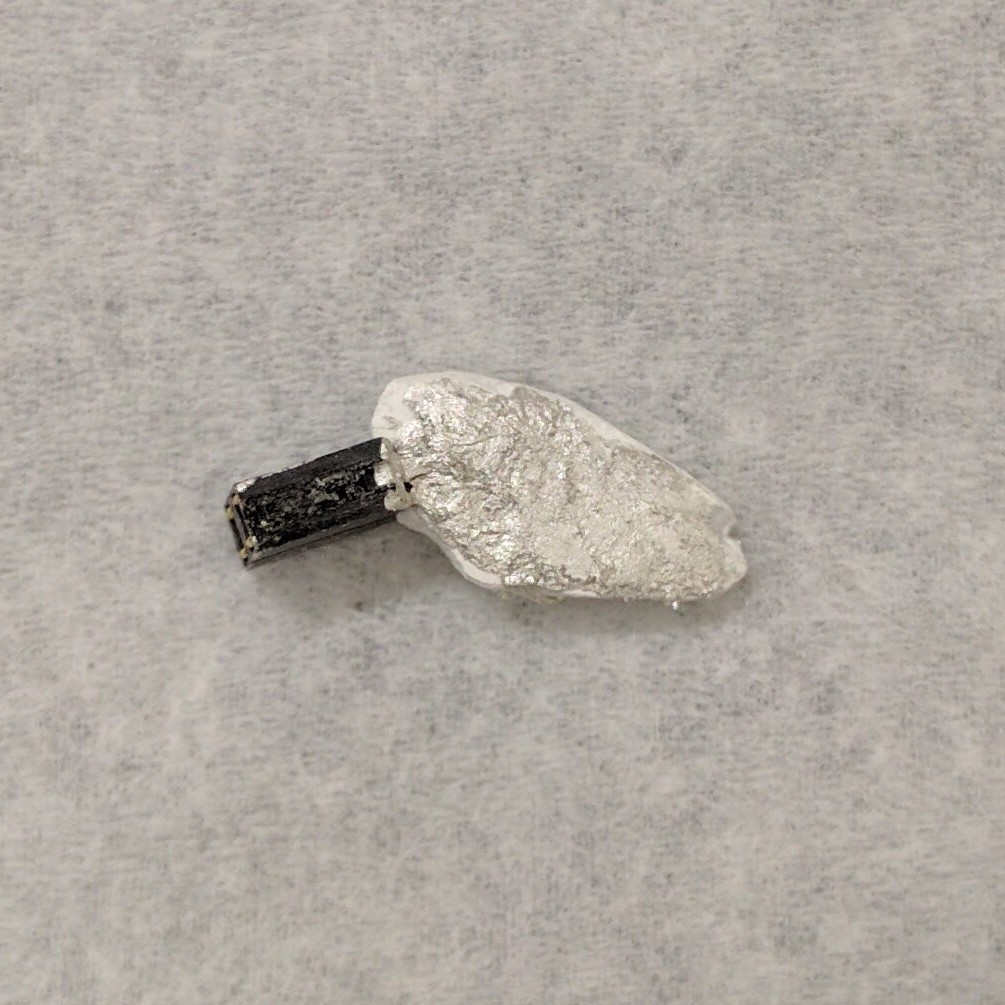
\includegraphics[width=\textwidth]{sample_complete.jpg}
		\caption{}
		\label{fig:sample:final}
	\end{subfigure}
	\begin{subfigure}{0.22\textwidth}
		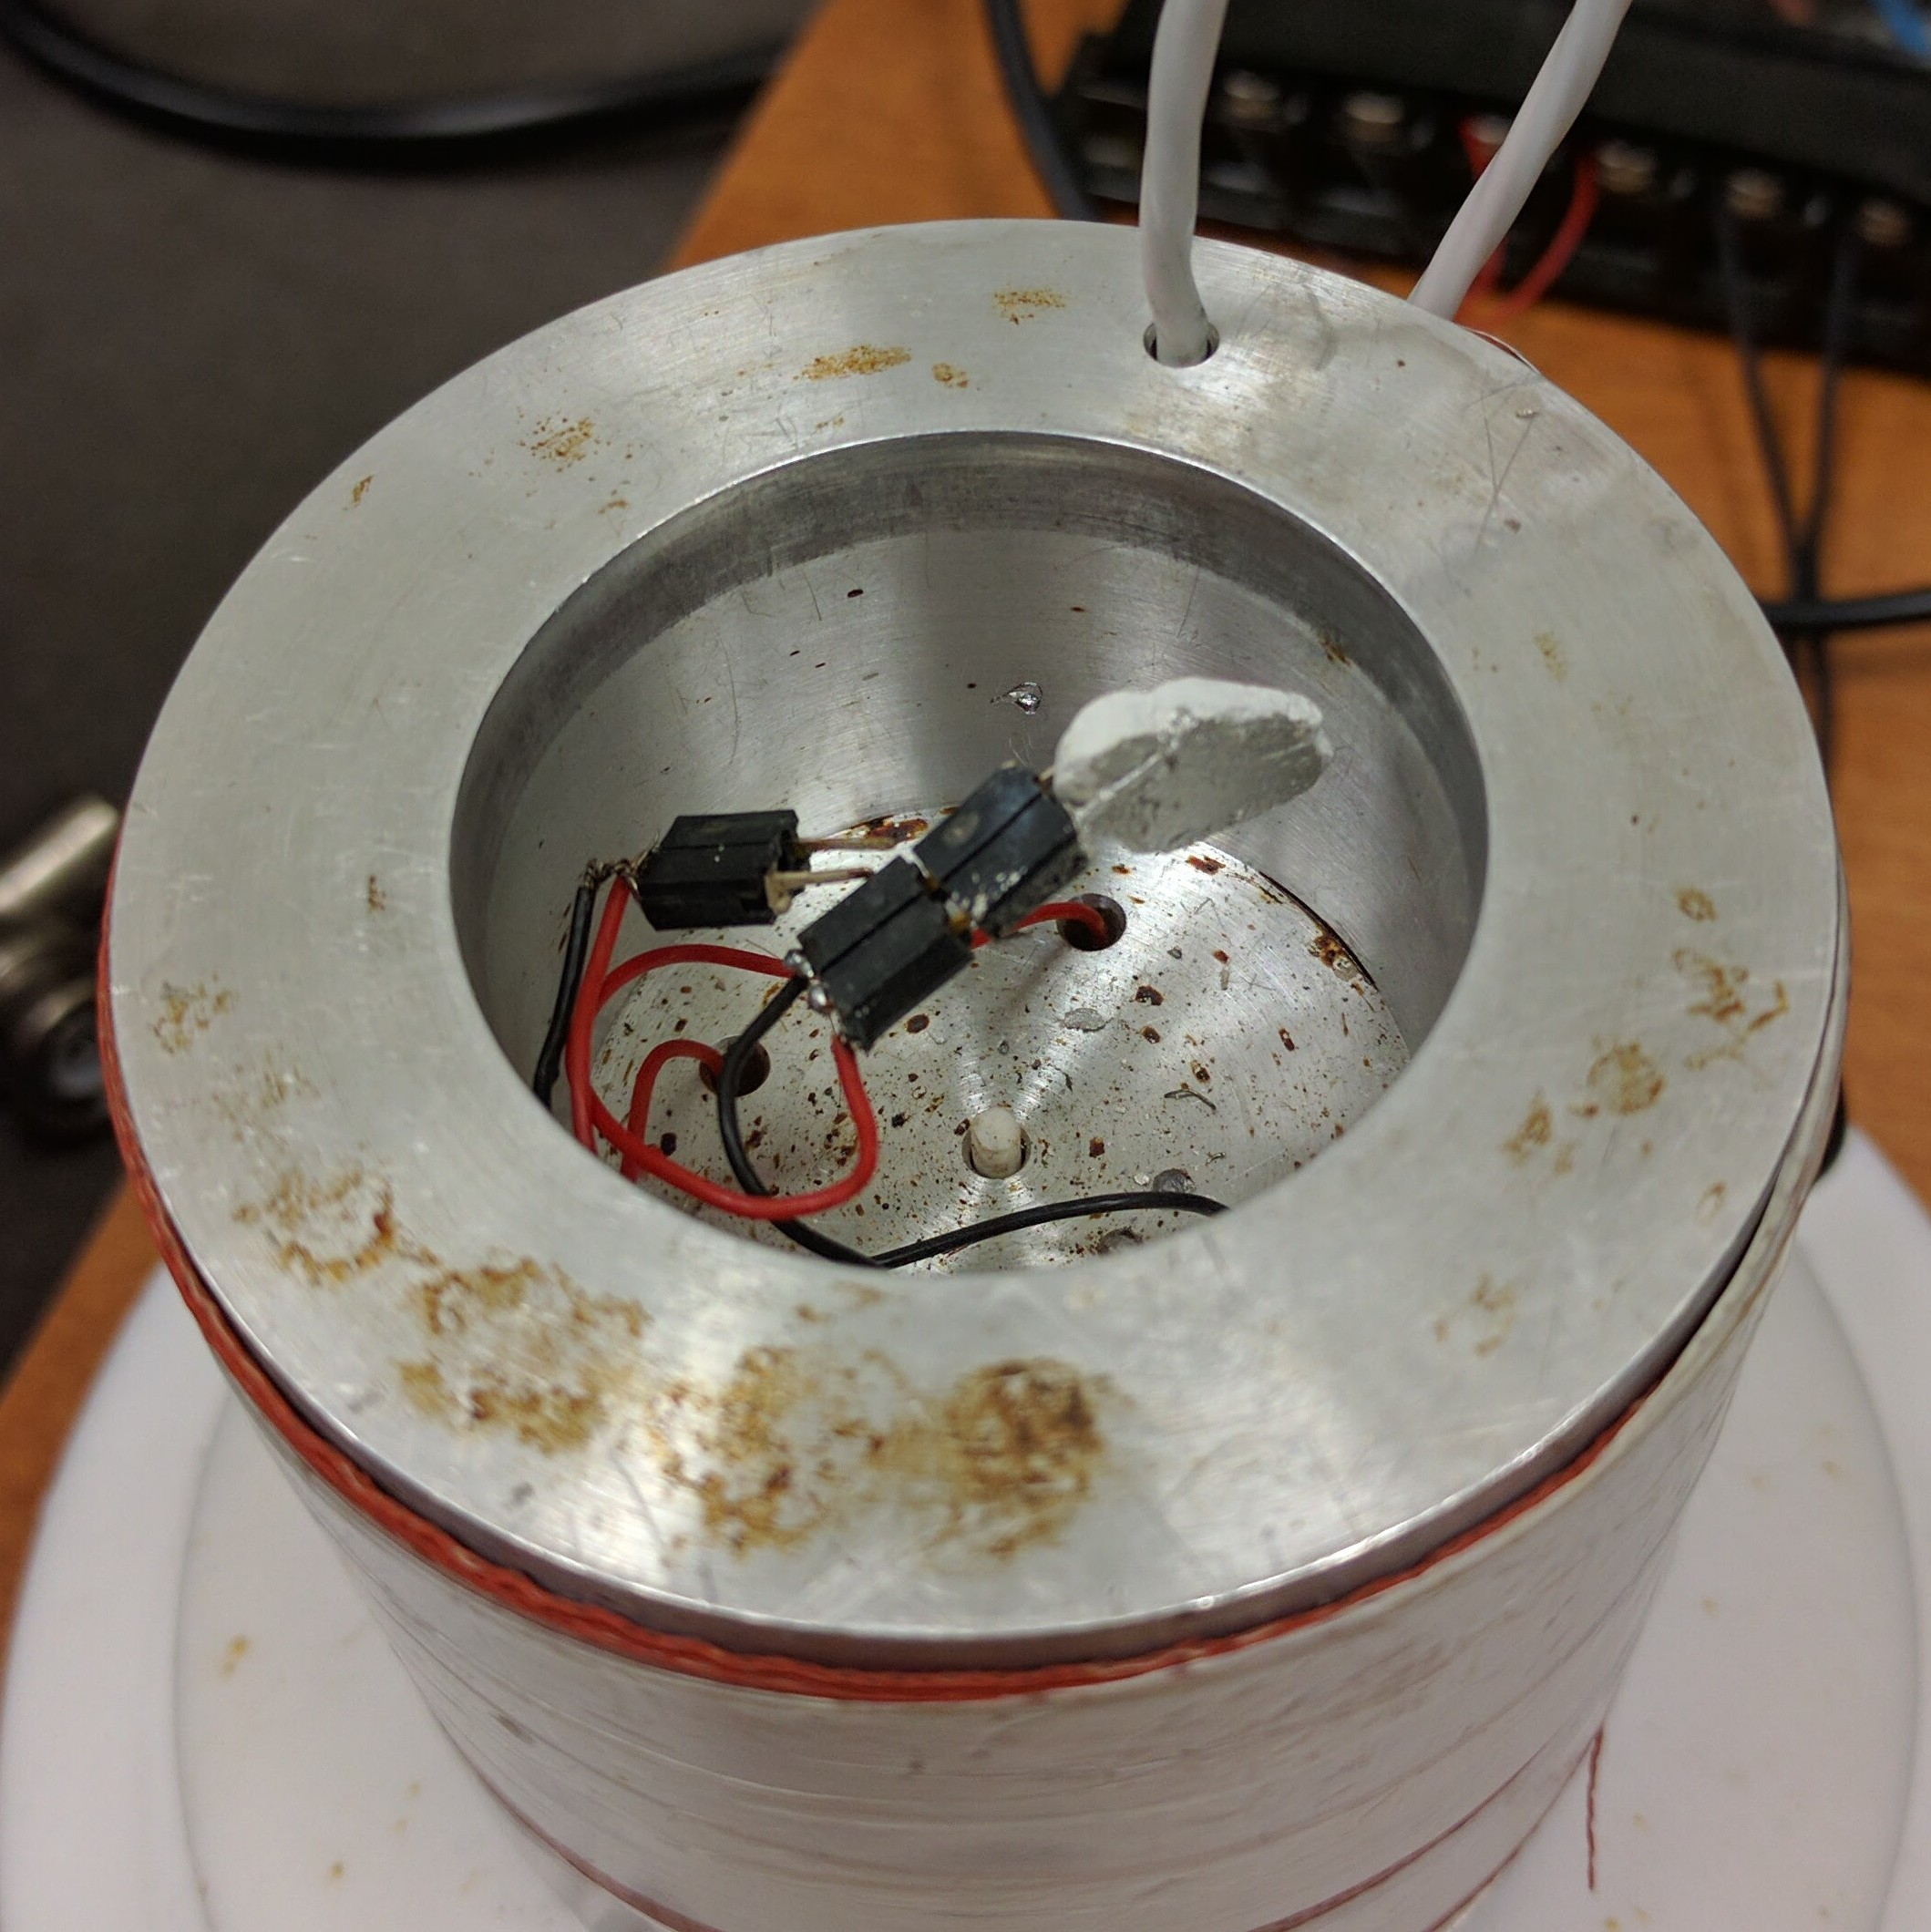
\includegraphics[width=\textwidth]{sample_inplace.jpg}
		\caption{}
		\label{fig:sample:inplace}
	\end{subfigure}
	\caption{Preparation of the Barium Titanate sample. Subfigures \ref{fig:sample:area} and \ref{fig:sample:thickness} show the images used to measure the thickness and the area of the sample. Subfigures \ref{fig:sample:final} and \ref{fig:sample:inplace} show the final sample, with the electrical connections attached by silver paint.}
	\label{fig:sample}
\end{figure}

Because we chose to maximize the area rather than creating a uniform (and easy to measure) geometric shape, we performed an indirect measurement of the area. Using a cell phone camera, we took an image with the sample and a ruler at the same distance. We used the photo editing tool GIMP to determine the surface area and thickness of the sample in pixels ($px$). We also measured the length of a section of the ruler to determine the $px$ to $mm$ conversion factor. From these measurements, we found that the area and thickness of the sample were:
\begin{gather}
	A_{sample} = 77.464 \pm 1.5470*10^{-2} ~mm^2  \nonumber \\
	d_{sample} = 1.8592 \pm 1.7820*10^{-3} ~mm	 \nonumber
\end{gather}
These values are consistent with our rough approximations made during the lab period. From these we find that our equation for the capacitance of this sample is:
\begin{gather}
	\begin{align}
		C = \frac{\epsilon A}{d} & = k \epsilon_0 \frac{77.464 \pm 1.5470*10^{-2} ~mm^2}{1.8592 \pm 1.7820*10^{-3} ~mm} \nonumber \\
		& = k*(3.2384*10^{-13} \pm 3.1902*10^{-16})~F \nonumber \\
		& = k*(0.32384 \pm 3.1902*10^{-4})~pF \nonumber
	\end{align}
\end{gather}
where k is the relative dielectric permeability of the sample. 


\subsection{Isolation of Extraneous Factors}\label{section:factors}

In order to accurately measure the resistance and capacitance of our samples, we need to account for any extraneous factors in our measurement apparatus which may distort the results. The two main factors we have isolated and accounted for are the internal resistance of the lock-in and the parasitic capacitance of our BNC cables. In order to isolate the internal resistance of the lock-in, we measured the lock-in voltage a number of known resistors with a known limiting resistance. Thus, by rearranging Ohm's Law, we can arrive at a simple expression for the internal resistance of the lock-in. We found the average value of this over many measurements to be:
\begin{gather}
	I = \frac{V_{output}}{R_{internal} + R_{limit} + R_{sample}} = \frac{V_{measured}}{R_{sample}} \nonumber \\
	\downarrow \nonumber \\
	\begin{align}
		R_{internal} 		& = \frac{V_{output}R_{sample}}{V_{measured}} - R_{sample} - R_{limit} \nonumber \\
		\bar{R}_{internal} 	& = 1028.7090 \pm 19.6005 \nonumber
	\end{align}
\end{gather}
We will use this value when evaluating the resistance of our VO$_2$ samples later in the report.

Similarly, we used a systematic approach to quantify the capacitance of our BNC cables. We connected the setup as if for a capacitance measurement, but instead of a BaTiO$_3$ sample we inserted an open-ended BNC cable. We measured the voltage across the lock-in for a number of different lengths of cable and then using the expression $C = \delta/(\omega*R_{int})$ found a value for the average capacitance per unit length:
\begin{gather}
	\frac{C}{1~meter} = 113.3195 \pm 2.5618~pF/m \nonumber
\end{gather}
This capacitance will add linearly with the capacitance of our samples, and is on a similar order, and so is important to be able to isolate this effect. Once these effects were accounted for, we 

\section{Measurements}
\subsection{Metal-Insulator Transition in $VO_{2}$}
We began with our study of the first order metal-insulator transition of $VO_{2}$. After tuning the lock in amplifier, we connected it to our sample to measure the voltage across the $VO_{2}$. We set the heater to increase the temperature of the sample chamber at a rate slow enough to allow for any time delay between the heating of the chamber and the heating of the sample itself. Since the sample is conductively heated, the temperature of the $VO_{2}$ itself may be lower than the temperature measured inside the chamber. Therefore, allowing the heater to increase the temperature at a slow enough rate ensures that the temperature read by the temperature sensor is consistent with that of the sample. As we increased the temperature we measured and recorded the temperature of and voltage across our $VO_{2}$ sample. The current in the circuit does not change so the variation in voltage as a function of temperature is due to the temperature dependence of the resistivity of the sample. To demonstrate this, we calculated the resistance, $R_{VO_{2}}$, of the sample from the voltage, $V_{out}$, across it using Eq.~\ref{Eq:VtoR}.

\begin{equation}\label{Eq:VtoR}
R_{VO_{2}} = \frac{V_{out}}{I} = \frac{V_{out} (R_{limit} + R_{internal})}{(V_{In} - V_{Out})} 
\end{equation}

where $V_{in}$ is the voltage output by the lock in amplifier, $R_{internal}$ is the internal resistance of the lock in amplifier, and $R_{limit}$ is the limiting resistance in the circuit which we set as $R_{limit} = 997 k\Omega$. For each value of voltage measured, we calculated the resistance of our sample and plotted this data as a function of temperature in Fig.~\ref{Fig:RvT1}.

\begin{figure}[H]
	\centering
	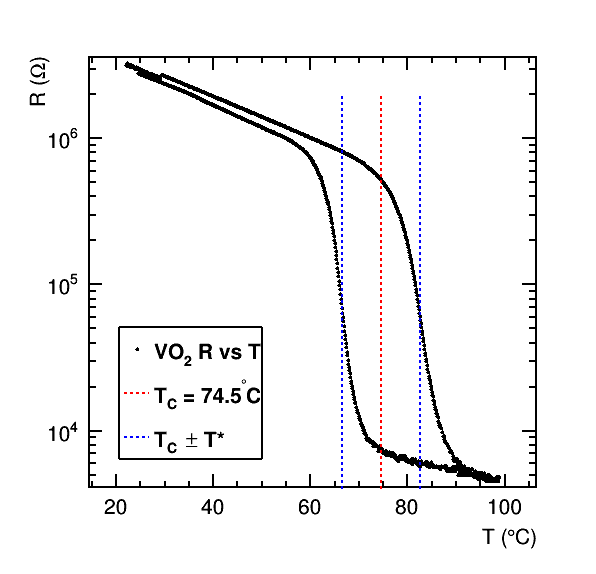
\includegraphics[width=0.4\textwidth]{VO2_RvT_withTC.png}
	\caption{Resistance vs Temperature Plot for $VO_{2}$ with Vertical Lines Identifying $T_{C}$ (Red) and $T_{C} \pm T^{*}$ (Blue)}
	\label{Fig:RvT1}
\end{figure}

The resistances of the sample are plotted on a logarithmic scale in order to better demonstrate at what temperature $V0_{2}$ exhibits a decrease in resistivity of a few orders of magnitude. As can be observed in Fig.~\ref{Fig:RvT1}, this drastic change in resistance occurs along two different curves. One of these curves is the change in resistance as the temperature of the sample was heated and the other curve is the resistance as the sample cooled down. The splitting of these curves was due to hysteresis and means that critical temperature must be found through a more analytical method. To find the transition point, we identified the inflection points of each curve. These points (identified in Fig.~\ref{Fig:RvT1} by vertical blue lines) indicate the coercive temperatures of the transition, $T_{C} \pm T*$. As the temperature of the sample increased, the metal-insulator transition occurred at $T_{C} + T* = 82.5 ^\circ C$, whereas when we decreased the temperature of the sample, hysteresis caused the transition to occur at $T_{C} - T* = 66.5 ^\circ C$. The critical temperature $T_{C}$ of the phase transition occurred at the average of these two points, $T_{C} = 74.5^\circ C$. At this temperature, we observed the resistivity of $VO_{2}$ change from $~10^{6}$ in the semiconducting phase to $~5 \times 10^3$ in its metallic phase, demonstrating a change in resistivity of about 2.5 to 3 orders of magnitude.

In addition to observing the transition point of the $VO_{2}$, we also observed its semiconducting properties at low temperatures, before it transitioned to its metallic phase. In this regime, the resistivity of the sample demonstrated the temperature dependence typical of a semiconductor, which behaves according to Eq.~\ref{Eq:SemiEGap}.

\begin{equation}\label{Eq:SemiEGap}
\rho = \rho_{0} e^{\frac{E_{g}}{2kT}}
\end{equation}

\noindent In this equation, $E_{g}$ is the energy gap, the energy difference between the valence band and conduction band of electrons. We tested that $VO_{2}$ exhibited semiconducting behavior at low temperatures by verifying the size of $E_{g}$. In order to calculate this value, we plotted the data on a $Log(\frac{\rho}{\rho_{0}})$ vs. $T^{-1}$ graph and fitted the data to a line. The data we collected is plotted as such in Fig.~\ref{Fig:RvT2}. Since we were testing the behavior of $VO_{2}$ in its semiconducting phase, we only fitted a line to the low temperature regime where it would exhibit such behavior.

\begin{figure}[H]
	\centering
	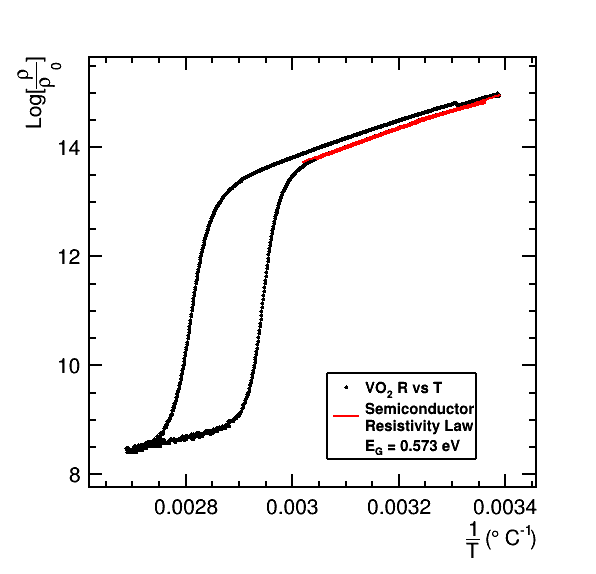
\includegraphics[width=0.4\textwidth]{VO2_LogRvTInv.png}
	\caption{$Log(\rho)$ vs. $\frac{1}{T}$ Plot to Find Semiconductor Energy Gap, $E_{g}$}
	\label{Fig:RvT2}
\end{figure}

\noindent The slope of this line is related to the energy gap as $E_{g} = 2k*(slope)$, where $k$ is Boltzmann's constant. We calculated the value of the band gap to be $E_{g} = 0.573 \pm 0.002 eV$, which we will see later is consistent with semiconducting behavior.

\subsection{Ferroelectric Transition in $BaTiO_{3}$}

The next phase transition that we studied was the second order ferroelectric transition of barium titanate, BaTiO$_{3}$. In this portion of the experiment, we hoped to observe the immediate emergence of an electric polarization in the BaTiO$_{3}$ at the transition temperature, $T_{C}$, known as the Curie temperature. This polarization comes about as a result of the shifting of atoms in a crystal of BaTiO$_{3}$, creating a dipole. As crystals of BaTiO$_{3}$ become dipoles in a large quantities, a sample of BaTiO$_{3}$ acts as a capacitor separating positive and negative charges on its surface. Therefore, to measure the properties of a ferroelectric phase transition in BaTiO$_{3}$, we used the lock-in amplifier to measure the capacitance across our sample of BaTiO$_{3}$.

To start, we again tuned the lock-in amplifier, and then set it to measure the voltage of the out-of-phase signal. As previously discussed, phasor theory says the voltage across a capacitor is $\approx 90^\circ$ out of phase with the signal output by the amplifier, so measuring this voltage provided us with the necessary information to analyze the capacitance of our BaTiO$_{3}$ sample. We recorded data of the voltage $V_{out}$ across our sample, versus its temperature, $T$. Using our measurements of the voltage, we could calculate the capacitance of the sample using Eq.~\ref{Eq:VtoC}.

\begin{equation}\label{Eq:VtoC}
C = \frac{1}{\omega R} \frac{1 - \sqrt{1 - 4(\frac{V_{out}}{V_{in}})^2 }}{2\frac{V_{out}}{V_{in}}}
\end{equation}

\noindent For our experiment, the input voltage of the lock-in amplifier was $V_{in} = 1.99V$, we set the frequency of the input signal as $f = \frac{\omega}{2\pi} = 25kHz$, and the resistance $R$ of the circuit was the internal resistance of the lock-in amplifier, $R_{internal}$.

\begin{figure}[H]
	\centering
	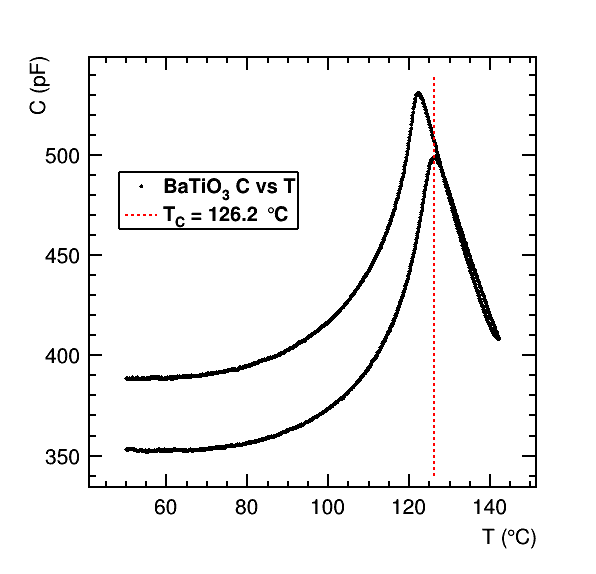
\includegraphics[width=0.4\textwidth]{BaTiO3_CvT_withTC.png}
	\caption{Resistance vs Temperature Plot for $BaTiO_{3}$ with a Vertical Line Identifying $T_{C}$ (Red)}
	\label{Fig:CvT1}
\end{figure}

\begin{figure}[H]
	\centering
	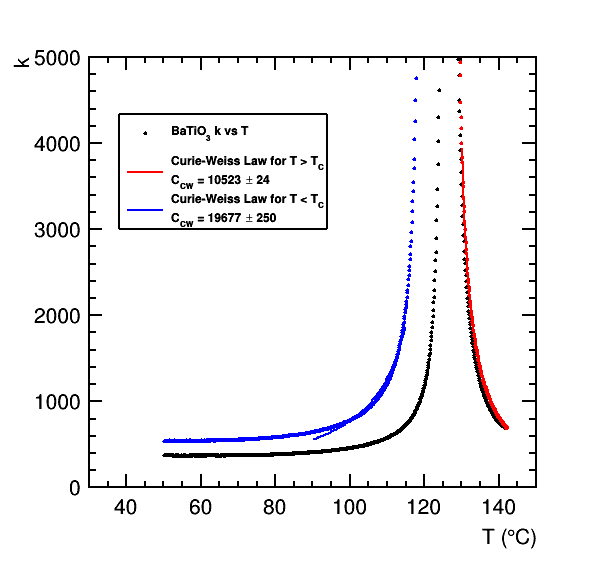
\includegraphics[width=0.4\textwidth]{BaTiO3_kvT.png}
	\caption{Relative Dielectric Constant vs Temperature Plot for $BaTiO_{3}$ with the Curie-Weiss Law both Above (Red) and Below (Blue) the Critical Temperature $T_{C}$}
	\label{Fig:kvT}
\end{figure}

\section{Theoretical Model}

\subsection{Metal-Insulator Transition of Vanadium Dioxide}

The theory behind metal insulator transitions is well studied \cite{phase_2}, and the specific properties of the Vanadium Dioxide transition have long been a topic of scientific interest \cite{manual, vo2_1, vo2_2}. In fact, it is the general consensus that the Metal-Insulator transition present in VO$_2$ can be described completely by the \textit{Mott insulator} model \cite{manual}. In such a Mott insulator, the coulomb repulsion between the electrons of the material in the same orbitals keeps them from conducting freely within the material at low (below $T_C$) temperatures. However, at sufficiently high temperatures, this barrier can be overcome and a signifigant current can flow. Thus, Mott proved, these materials will experience a transition from a low-temperature insulating state to a high-temperature conductive state.

The transition does not happen for the entire bulk material at once, however. Instead, like water freezing, 'nucleation' sites form somewhat at random within the material. These metal zones grow outwards from their points of origin as the temperature grows above $T_C$. At some point, these zones will connect to form a single unbroken conductive path through the material and the \textit{percolation transition} is said to have taken place \cite{perc}. For a 2D system, which is a good approximation for our thin VO$_2$ films, the spanning probability is found to be $\rho_c = 0.592 7460 \pm 0.000 0005 $ \cite{perc,perc2}. This means that, on average, when $59\%$ of the VO$_2$ has transitioned into a metal the entire length of the system will be spanned and the percolation transition will be complete.

\begin{figure}[H]
	\centering
	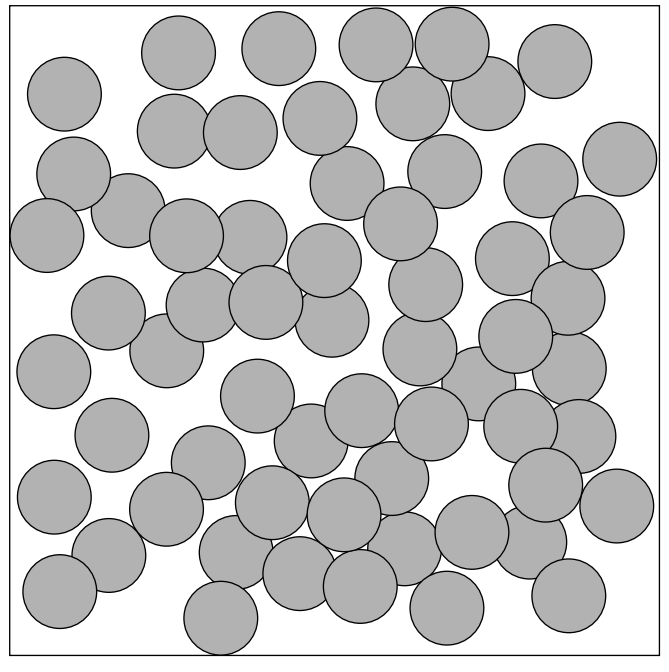
\includegraphics[width=0.25\textwidth]{percolation.png}
	\caption{Percolation of a general lattice with circular transition zones. In a MIT, these darker zones would represent the metal zones which, once connected all the way through the sample, form a single conductive path. Image courtesy of \cite{perc}.}
	\label{fig:perc}
\end{figure}

The properties of VO$_2$ are well documented, and the known values for the transition parameters can be found in the table below:

\begin{Huge}
TOM ADD SOMETHING HERE
\end{Huge}

\noindent In the coming sections, we will compare these known results with the results from our own experiments.

\subsection{Ferroelectric Transition of Barium Titanate}

\section{Comparison of Theory and Experiment}

\subsection{Metal-Insulator Transition of Vanadium Dioxide}

\subsection{Ferroelectric Transition of Barium Titanate}

\section{Discussion and Conclusions}

During the course of our measurements, we found that even after repeated tuning of the phase and replacement of various cables the lock-in would drift erratically. During some periods the equipment would remain stable for hours before suddenly beginning to drift with no obvious external cause. Additionally, the internal resistance of the lock-in which we observed was almost double its original value of $600~\Omega$, which also indicates some internal damage to the equipment. We were able to take good measurements in spite of this, but further investigation of the cause and possible solutions to this problem should be investigated if this lab is to be performed by future students. 

\section{Author Contributions}

Both authors believe that the work for this project was split equally, and each offered valuable insight to every section of this report. However, the sections when divided up by principle author are as follows:

\noindent \textbf{Joshua LaBounty}:
\begin{enumerate}
	\item Section 1: Introduction
	\item Section 2: Review of Previous Work
	\item Section 3: Experimental Setup
	\item Appendix \ref{section:fourprobe}: Four Probe Method
\end{enumerate}

\noindent \textbf{Thomas Krahulik}:
\begin{enumerate}
	\item Section 4: Measurements
	\item Appendix \ref{section:root}: Validation of the $\chi^2$ Minimization in ROOT
\end{enumerate}

\noindent Lab time was also split equally, with one partner often taking measurements while the other developed the analysis software used in this report.

\begin{thebibliography}{6}
	
	\bibitem{milissinos}
	A.C. Melissinos, Experiments in Modern Physics (Academic Press, NY, 1966).
	
	\bibitem{bevington}
	Philip R. Bevington and D. Keith Robinson, Data Reduction and Error Analysis 3rd edition (McGraw-Hill, 2003).
	
	\bibitem{manual}
	Mihaly, Laszlo and Gurvitch, Micheal. Phase Transitions: Metal-Insulator Transition in VO$_2$ and Ferroelectric Transition in BaTiO$_3$. (Stony Brook University, Nov. 14, 2014)
	
	\bibitem{phase_1}
	Hadley, P. Advanced Solid State Physics: Landau theory of second order phase transitions. (Institute of Solid State Physics, 2011). \url{http://lampx.tugraz.at/~hadley/ss2/landau/second_order.php}
	
	\bibitem{modern_apps}
	M. Gittrman, V. Halpern, “Phase Transitions; A brief account with modern applications” World
Scientific, (2004)

	\bibitem{physics_of_phase}
	P. Papon, J. Leblond, P.H.E. Meijer, “The Physics of Phase Transitions”, Springer, (2001)
	
	\bibitem{phase_2}
	V. Dobrosavljevic, “Introduction to Metal-Insulator Transitions” (2011), arXiv:1112.6166v1
	
	\bibitem{phase_history}
	Jaeger, G. The Ehrenfest Classification of Phase Transitions: Introduction and Evolution. Archive for History of Exact Sciences. (1 May 1998). doi:10.1007/s004070050021.
	
	\bibitem{gibbs}
	Gibbs, J.W. On the Equilibrium of Heterogeneous Substances. Connecticut Academy of Arts and Sciences, 1874. \url{https://archive.org/details/Onequilibriumhe00Gibb}
	
	\bibitem{thirdorder}
	E.C. Ekuma; G.C. Asomba and M.I. Okoye. Thermodynamics of Third Order Phase Transition: A Solution to the Euler -- Lagrange Equations. 	Physica B: Condensed Matter, Volume 405, Issue 9, Pages 2290-2293 (May 2010).
	
	\bibitem{mott}
	Mott, N.F. Metal-Insulator Transitions. University of Cambridge (1990).
	
	\bibitem{switching}
	Chudnovskiy, F., Luryi, S., and Spivak B. Switching device based on first-order metal-insulator transition induced by external electric field. SUNY Stony Brook (2002).
	
	\bibitem{memory}
	Elliman, Robert. The metal-insulator transition (MIT) and its application as a selector device for nonvolatile memory. Australian National University (June 2016).
	
	\bibitem{cosmo}
	Ryden, B. Introduction to Cosmology. Addison-Wesley (2002).
	
	\bibitem{cosmo2}
	Starobinsky, A.A. Dynamics of phase transition in the new inflationary universe scenario and generation of perturbations. Physics Letters B Volume 117, Issues 3–4, Pages 175-178 (November 1982).
	
	\bibitem{cosmo3}
	Gene F. Mazenko, William G. Unruh, and Robert M. Wald. Does a phase transition in the early universe produce the conditions needed for inflation? Phys. Rev. D 31, 273 (January 1985).
	
	\bibitem{cosmo4}
	Daile La and Paul J. Steinhardt. Extended Inflationary Cosmology. Phys. Rev. Lett. 62, 376, 1066 (1989).
	
	\bibitem{cosmo5}
	J. Barriga, E. Gaztañaga, M.G. Santos and S. Sarkar.On the APM power spectrum and the CMB anisotropy: evidence for a phase transition during inflation? MNRAS 324 (4): 977-987 (2001). 
	
	\bibitem{superconductor}
	Kleinert, H. Order of superconductive phase transition. Condensed Matter Physics, Vol. 8, No. 1(41), pp. 75–86 (2005).
	
	\bibitem{supercond2}
	Maximenko, Y. Superconducting phase transition. University of Illinois, Urbana-Champaign (2011).
	
	\bibitem{supercond3}
	Cyrot, M. Ginzburg-landau theory for superconductors. Rep. Prog. Phys., 36:103 (1973).
	
	\bibitem{rapheal}
	Cervantes, R. A Compact Magnetic Field Cloaking Device. Stony Brook University (2015).
	
	\bibitem{magnets}
	Wilson, M.N. Superconducting magnets. Clarendon Press; Oxford (1983).
	
	\bibitem{quantum_super}
	Lev B. Ioffe, Vadim B. Geshkenbein, Mikhail V. Feigel'man, Alban L. Fauchere, and Gianni Blatter. Environmentally decoupled sds-wave Josephson junctions for quantum computing. Nature 398, 679-681 (22 April 1999).
	
	\bibitem{quantum_super2}
	MJ Feldman and X. Zhou. SUPERCONDUCTING QUANTUM COMPUTING WITHOUT SWITCHES. University of Rochester (2002).
	
	\bibitem{trains}
	K Ushio and K Hiroshi. High speed train utilizing hard superconductor. US Patent 3,662,689 (1972)
	
	\bibitem{capacitors}
	Waugh, Mark D. Design solutions for DC bias in multilayer ceramic capacitors. Electronic Engineering Times.(2010)
	
	\bibitem{thermals}
	Vipul Bansal, Pankaj Poddar, Absar Ahmad, and Murali Sastry. Room-Temperature Biosynthesis of Ferroelectric Barium Titanate Nanoparticles. J. Am. Chem. Soc., 128 (36), pp 11958–11963 (2006).
	
	\bibitem{vo2_1}
	C. N. Bergland and H. J. Guggenheim, “Electronic properties of VO2 near the semiconductor metal transition”, Phys. Rev. 185 (3), pp. 1022-1033 (1969).
	
	\bibitem{vo2_2}
	M. Gurvitch, Serge Luryi, A. Polyakov, A. Shabalov, “Nonhysteretic Phenomena in the Metal Semiconductor Phase-Transition Loop of VO2 Films for Bolometric Sensor Applications”, IEEE Transactions on Nanotechnology 9, pp. 647-652 (2010).
	
	\bibitem{perc}
	Harvey Gould, Jan Tobochnik, and Wolfgang Christian. Chapter 13: Percolation. (April 2001).
	
	\bibitem{perc2}
	Robert M. Ziff, “Spanning probability in 2D percolation,” Phys. Rev. Lett. 69, 2670 (1992).

\end{thebibliography}

\begin{appendix}

\section{Four Probe Method}\label{section:fourprobe}

Because the resistances of our samples may be small (or comparable to our contact resistances), we have chosen to employ the four-probe resistance measurement method shown in Figure \ref{fig:ResistanceMeasurements} over the simpler two-probe method we employed extensively in PHY 335. The advantage of the four probe method is that it effectively removes the influence of the contact resistances from our measurements. The reason for this is as follows. In a two-probe sensor, where the current and the voltage leads connect at the same point, the full ammeter current flows through the contacts of the voltmeter. This means that the voltage drop across the ammeter will be equal to $V = I_{Ammeter}*(R_{Sample} + 2R_{Contact})$. However, when the connections of the voltmeter and ammeter are separated as in the four-probe method, the full current will only flow through the ammeter connections (which will not alter the measurement of current). The flow of current through the voltmeter connections will then only be the small ($\sim pA$) current through the voltmeter itself, limited by its large internal resistance. Now, the voltmeter voltage is $V = I_{Ammeter}*R_{Sample} + I_{Voltmeter} + 2R_{Contact} \approx I_{Ammeter}*R_{Sample}$. So long as the contact resistances are much lower than the internal resistance of the measurement device, then their effect on the measurement can be neglected. This method will allow us to examine the resistances of our samples without having to worry about the effect of the quality of our connections (in our lock in, the "Measuring input" functions as the voltmeter while the "Oscillator voltage out" acts as the ammeter).

\section{Validation of the $\chi^2$ Minimization in ROOT} \label{section:root}
For this experiment, we used ROOT, a c++ based data analysis software, to plot and fit functions to our data. To verify that ROOT calculates a correct value for $\chi^{2}$, we performed a hand calculation cross check with a simple set of data. The data set we used for this cross check was $\{ (11.0 \pm 0.0, 23.0 \pm 0.5), (14.0 \pm 0.0, 25.0 \pm 0.5), (20.0 \pm 0.0, 35.0 \pm 0.5), (25.0 \pm 0.0, 39.0 \pm 0.5) \}$. We plotted this data and fit it to a linear function $f(x) = [0] + [1]*x$. This plot is shown in Fig.~\ref{Fig:rootproof}.
\begin{figure}[H]
	\centering
	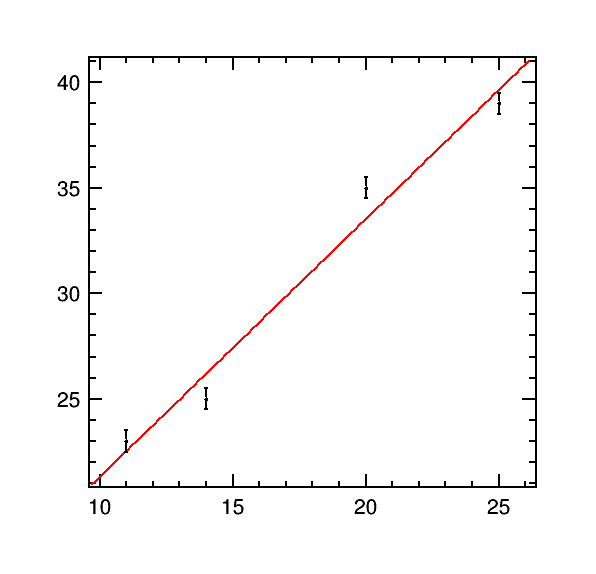
\includegraphics[width=0.4\textwidth]{rootproof.png}
	\caption{Sample Data Fitted to a Line}
	\label{Fig:rootproof}
\end{figure}
The function obtained from this fit was $f(x) = 9.11111 + 1.22222x$ with a chi-squared of $\chi ^{2} = 16.8889$. We then performed a hand calculation of the $\chi ^{2}$ using Eq.~\ref{eq:chisq}.
\begin{gather}\label{eq:chisq}
\chi ^{2} = \sum \frac{(f(x_i) - y_i)^{2}}{\sigma_i^2}
\end{gather}
When performing this hand calculation we also obtained a value of $\chi ^{2} = 16.8889$, verifying ROOT's ability to calculate $\chi ^{2}$.
\begin{align*}
\chi ^{2} =& \frac{(f(11.0) - 23.0)^{2}}{(0.5)^2} + \frac{(f(14.0) - 25.0)^{2}}{(0.5)^2} \\
&+ \frac{(f(20.0) - 35.0)^2}{(0.5)^2} + \frac{(f(25.0) - 39.0)^{2}}{(0.5)^2} \\
&= 16.8889
\end{align*}

\section{Analysis Code} \label{section:analysis_code}
All of the analysis code used for this lab can be found in the following git repository: 
\begin{verbatim}
https://github.com/jlabounty/SeniorLab/tree
/master/PhaseTransitions/
\end{verbatim}

\end{appendix}

\end{document}
